\documentclass[tikz,border=10pt,multi=tikzpicture]{standalone}
\usepackage{amsmath}
\usepackage{xcolor}
\definecolor{mainblue}{HTML}{001158}
\definecolor{accent}{HTML}{8592bc}
\definecolor{lightaccent}{HTML}{e7e9f2}
\definecolor{normalcolor}{HTML}{2a9d8f}
\definecolor{shearcolor}{HTML}{c1121f}
\definecolor{loadcolor}{HTML}{e67e22}

\begin{document}

% ---------- PAGE 1: 1D tension bar with Hooke's law ----------
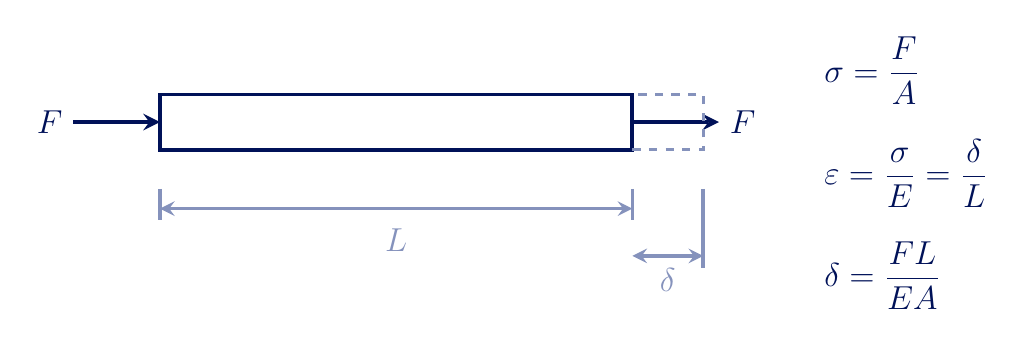
\begin{tikzpicture}[>=stealth, line width=1.3pt, font=\large]
  % original bar
  \draw[mainblue, line width=1.4pt] (0,0) rectangle (6,0.7);

  % force arrows (tension, pulling outward)
  \draw[mainblue, ->, line width=1.6pt] (-1.1,0.35) -- (0,0.35);
  \node[mainblue] at (-1.4,0.35) {$F$};
  \draw[mainblue, ->, line width=1.6pt] (6,0.35) -- (7.1,0.35);
  \node[mainblue] at (7.4,0.35) {$F$};

  % dimension L (original length)
  \draw[accent] (0,-0.5) -- (0,-0.9);
  \draw[accent] (6,-0.5) -- (6,-0.9);
  \draw[accent, <->] (0,-0.75) -- (6,-0.75);
  \node[accent] at (3,-1.15) {$L$};

  % dashed stretched outline + elongation dimension
  \draw[accent, dashed, line width=1pt] (6,0) -- (6.9,0) -- (6.9,0.7) -- (6,0.7);
  \draw[accent] (6.9,-0.5) -- (6.9,-1.5);
  \draw[accent, <->] (6,-1.35) -- (6.9,-1.35);
  \node[accent] at (6.45,-1.65) {$\delta$};

  \node[mainblue, font=\large, anchor=west] at (8.3,1.0) {$\sigma = \dfrac{F}{A}$};
  \node[mainblue, font=\large, anchor=west] at (8.3,-0.3) {$\varepsilon = \dfrac{\sigma}{E} = \dfrac{\delta}{L}$};
  \node[mainblue, font=\large, anchor=west] at (8.3,-1.6) {$\delta = \dfrac{FL}{EA}$};
\end{tikzpicture}

% ---------- PAGE 2: Querkraftprofil F_q(x) for the q0-Kragarm ----------
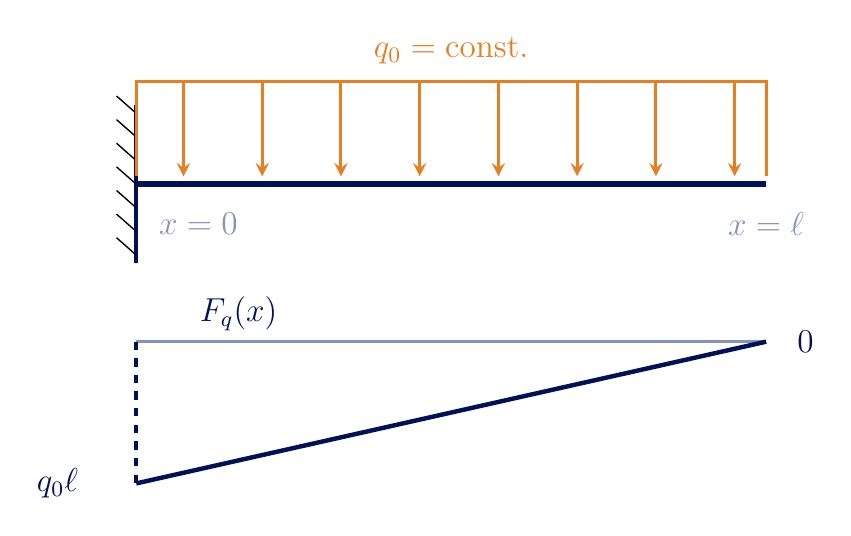
\begin{tikzpicture}[>=stealth, line width=1.3pt, font=\large]
  % wall / fixed support
  \draw[mainblue, line width=1.5pt] (0,1.0) -- (0,-1.0);
  \foreach \y in {-0.9,-0.6,...,0.9} {
    \draw[line width=0.5pt] (0,\y) -- (-0.25,\y+0.22);
  }

  % beam
  \draw[mainblue, line width=2pt] (0,0) -- (8,0);

  % distributed load q0 (uniform, downward arrows, closed box)
  \draw[loadcolor, line width=1.1pt] (0,0.1) -- (0,1.3) -- (8,1.3) -- (8,0.1);
  \foreach \x in {0.6,1.6,...,7.6} {
    \draw[loadcolor, ->, line width=1.1pt] (\x,1.3) -- (\x,0.1);
  }
  \node[loadcolor] at (4.0,1.7) {$q_0 = \text{const.}$};

  \node[accent, anchor=west] at (0.15,-0.5) {$x=0$};
  \node[accent] at (8,-0.5) {$x=\ell$};

  % Fq(x) diagram: linear, max q0*l at the wall, 0 at the free end
  \draw[accent] (0,-2.0) -- (8,-2.0);
  \draw[mainblue, line width=1.6pt] (0,-3.8) -- (8,-2.0);
  \draw[mainblue, dashed] (0,-2.0) -- (0,-3.8);
  \node[mainblue] at (1.3,-1.65) {$F_q(x)$};
  \node[mainblue] at (-1.0,-3.8) {$q_0\ell$};
  \node[mainblue] at (8.5,-2.0) {$0$};
\end{tikzpicture}

% ---------- PAGE 3: stress distribution over the cross-section height ----------
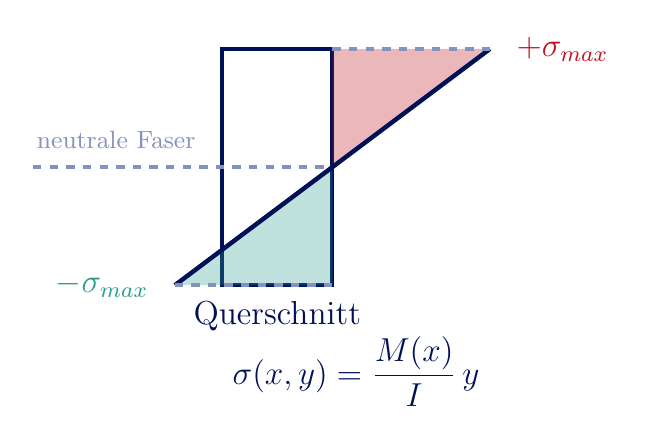
\begin{tikzpicture}[>=stealth, line width=1.3pt, font=\large]
  % cross-section (rectangle), y up, right edge at x=1.4
  \draw[mainblue, line width=1.4pt] (0,-1.5) rectangle (1.4,1.5);
  \draw[accent, dashed] (-2.4,0) -- (1.4,0);
  \node[accent, anchor=south east] at (-0.2,0.1) {\small neutrale Faser};
  \node[mainblue] at (0.7,-1.9) {Querschnitt};

  % stress distribution: positive (tension) to the right, negative (compression) to the left of the zero axis
  \fill[shearcolor, opacity=0.3] (1.4,0) -- (1.4,1.5) -- (3.4,1.5) -- cycle;
  \fill[normalcolor, opacity=0.3] (1.4,0) -- (1.4,-1.5) -- (-0.6,-1.5) -- cycle;
  \draw[mainblue, line width=1.6pt] (3.4,1.5) -- (1.4,0) -- (-0.6,-1.5);
  \draw[accent, dashed] (1.4,1.5) -- (3.4,1.5);
  \draw[accent, dashed] (1.4,-1.5) -- (-0.6,-1.5);

  \node[shearcolor, anchor=west] at (3.6,1.5) {$+\sigma_{max}$};
  \node[normalcolor, anchor=east] at (-0.8,-1.5) {$-\sigma_{max}$};

  \node[mainblue, font=\large] at (1.7,-2.6) {$\sigma(x,y) = \dfrac{M(x)}{I}\,y$};
\end{tikzpicture}

\end{document}
